\documentclass[11pt, xcolor=dvipsnames, aspectratio=43]{beamer}
\usetheme{CambridgeUS}
\useoutertheme{infolines}
%\usecolortheme{beaver}
\usepackage[utf8]{inputenc}
\usepackage[italian]{babel}
\usepackage{amsmath}
\usepackage{amsfonts}
\usepackage{amssymb}
\usepackage{graphicx}
\usepackage{physics}
\usepackage{circuitikz}
\usepackage{hyperref}
\usepackage{siunitx}
\usepackage{booktabs}
\usepackage{pgfplots}
\pgfplotsset{compat=1.17}
\usepackage[mode=buildnew]{standalone}
\usepgfplotslibrary{fillbetween}
\usetikzlibrary{pgfplots.groupplots}

\useinnertheme{circles}

\definecolor{UBCblue}{rgb}{0.7, 0, 0} % UBC Blue (primary)
\usecolortheme[named=UBCblue]{structure}


\newcommand{\fourier}[1]{\mathcal{F}\left\{#1\right\}}
\newcommand{\bs}[1]{\boldsymbol{#1}}

\title{Risposta impulsiva di un circuito RLC}
\subtitle{Analisi della risposta impulsiva di un circuito RLC serie nel dominio del tempo e della frequenza}
\author{Nicolò Montalti - 933833}
\date{14/06/2021}
\setbeamercovered{invisible} 
%\setbeamertemplate{navigation symbols}{} 
%\logo{} 
%\institute{Università di Bologna} 
\subject{Laboratorio di elettromagnetismo e ottica} 
\begin{document}

\begin{frame}
\maketitle
\end{frame}

\section{Panoramica dell'esperienza}
\begin{frame}{Panoramica dell'esperienza}
\begin{block}{Scopo}
Determinare, attraverso un'analisi nel dominio del tempo e della frequenza, le grandezza caratteristiche $\omega_0$ e $\gamma$ di un circuito RLC serie.
\end{block}
\pause
\begin{block}{Metodo}
\begin{enumerate}[<+->]
\item{Stimolo del circuito con un impulso;}
\item{analisi nel dominio del tempo di $V_C$;}
\item{trasformata di Fourier (FFT) dei dati;}
\item{analisi nel dominio della frequenza.}
\end{enumerate}
\end{block}
\end{frame}

\section{Circuito}
\begin{frame}{Schema del circuito}
\centering
\begin{circuitikz}[scale = 1.2]
\draw (0,0)
to[V=$V_G$] (0,2) % The voltage source
to[R=$R_G$] (0,4)
to[R=$R$] (4,4) % The resistor
to[C=$C$] (4,0) % Capacitor One
to[L=$L$] (2,0) %Inductor One
to[R=$R_L$] (0,0)
;
\draw (4,1)
to[short, -*] (5,1)
to[open, l_=$V_C$] (5,3)
to[short, *-] (4,3)
;
\end{circuitikz}

\end{frame}

\section{Comportamento atteso}
\begin{frame}{Leggi del circuito RLC}
\begin{itemize}

\item<1->{
Il comportamento di un circuito RLC è descritto dall'equazione
\[
\dv[2]{V_C}{t} + \gamma \dv{V_C}{t} + \omega_0^2 V_C = \omega_0^2 V_G(t)
\]
}

\item<2>{
Applicando l'operatore \alert{trasformata di Fourier} si può definire la \alert{funzione di trasferimento}
\[
H(\omega) = \frac{\fourier{V_C}}{\fourier{V_G}} = \frac{1}{1 - \left(\frac{\omega}{\omega_0}\right)^2 + j \frac{\gamma \omega}{\omega_0^2}}
\]
}
\end{itemize}
\end{frame}

\begin{frame}{Stimolo impulsivo}
\begin{itemize}
\item<1->{
Il circuito è stato stimolato con un segnale impulsivo $V_G(t) = V_0 \delta(t)$
}

\item<2->{
La risposta attesa nel dominio del \alert{tempo} era
\[
V_C(t) = Ae^{- \gamma t / 2}\sin{(\omega_p t)} \qquad \qquad \omega_p = \sqrt{\omega_0^2 - \gamma^2 / 4}
\]
}
\item<3->{
mentre nel dominio della \alert{frequenza} si verifica che
\[
H(\omega) = \frac{\fourier{V_C}}{\fourier{V_G}} = \frac{\fourier{V_C}}{V_0} =  \frac{1}{1 - \left(\frac{\omega}{\omega_0}\right)^2 + j \frac{\gamma \omega}{\omega_0^2}}
\]
}

\end{itemize}
\end{frame}

\section{Apparato sperimentale}
\begin{frame}{Parametri dell'apparato sperimentale}
\begin{itemize}
\item<1-> Parametri del circuito
\begin{itemize}
\item<1-> {$R = \SI{35.31 \pm 0.05}{\ohm}$, $C=\SI{32.0(3)}{\nano\farad}$, $L= \SI{10.17 (10)}{\milli\henry}$, $R_L = \SI{41.41 \pm 0.05}{\ohm}$, $R_G = \SI{50}{\ohm}$}
\item<1-> $\gamma^\text{exp} = \SI{12.46(12)}{\kilo\hertz}$, $\omega_0^\text{exp} = \SI{55.4(4)}{\kilo\hertz}$
\end{itemize}

\item<2-> Parametri del generatore
\begin{itemize}
\item<2-> $V_0 = \SI{5}{\volt}$
\item<2-> durata impulso: \SI{0.5}{\micro\second}
\item<2-> intervallo tra impulsi successivi: \SI{2}{\milli\second} 
\end{itemize}

\item<3-> Parametri di campionamento
\begin{itemize}
\item<3-> segnali campionati: $V_G$ (range $\pm\SI{10}{\volt}$) e $V_C$ (range $\pm\SI{0.2}{\volt}$)
\item<3-> frequenza di campionamento: \SI{500}{\kilo\hertz}
\item<3-> 800 campioni (durata \SI{1.6}{\milli\second})
\item<3-> trigger su $V_G$ (slope: rising, level: \SI{1}{\volt})
\end{itemize}
\end{itemize}

\end{frame}

\section{Risultati}
\begin{frame}{Dominio del tempo}
\begin{center}
\includegraphics<1>[scale=0.9]{Plottime}
\includegraphics<2>[scale=0.9]{Plottime_arrow}
\end{center}
\end{frame}

\begin{frame}{Dominio della frequenza: ampiezza e fase}
\begin{center}
\includegraphics<1>[scale=0.9]{Plotfreqs}
\includegraphics<2>[scale=0.9]{Plot_freqs_arrow}
\end{center}
\end{frame}


\begin{frame}{Dominio della frequenza: parte reale e immaginaria}
\centering
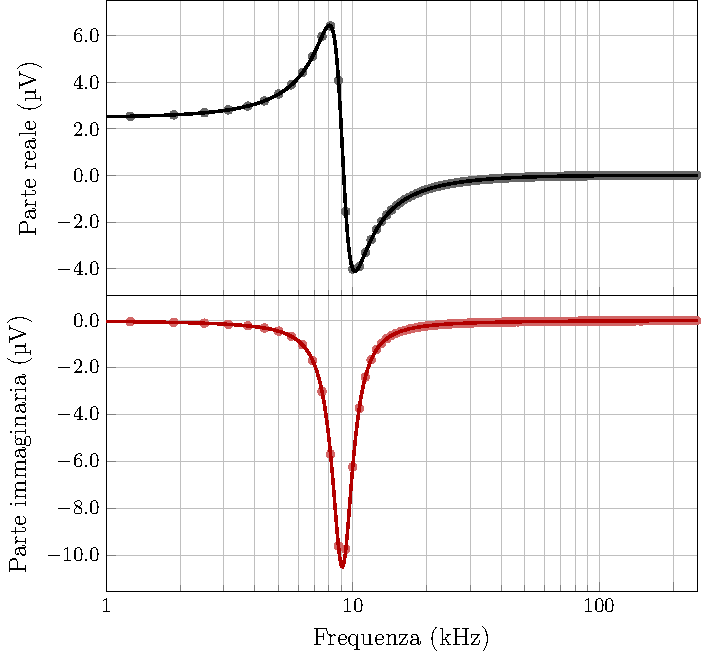
\includegraphics[scale=0.68]{Real_Imag}
\end{frame}


\begin{frame}{Procedura di fit}
\begin{itemize}[<+->]
\item Per tenere conto dello \alert{sfasamento} dovuto al trigger si è aggiunto un parametro $t_0$ alle funzioni da fittare.
\begin{itemize}
\item Il fit nel dominio del tempo è stato eseguito sulla funzione $V_C(t+t_0)$.
\item Ricordando che $\fourier{f(t+t_0)} =  \fourier{f(t)} e^{j\omega t_0}$, il fit nel dominio del tempo è stato eseguito sulla funzione $ H(\omega) e^{j\omega t_0}$.
\end{itemize}

\item Dal fit nel dominio del tempo è stato stimato un errore sui dati raccolti \alert{$\sigma_{V_C} = \SI{30}{\micro\volt}$}, che è stato propagato nel dominio della frequenza.

\item Entrambi hanno restituito un $R^2 = 1.00$, il secondo inoltre un $\tilde{\chi}^2 = 1.06$.

\end{itemize}

\end{frame}

\begin{frame}{Risultati}
\begin{center}
\begin{tabular}{lccc}
\toprule
Misura & $\omega_0$ (\si{\kilo\hertz}) & $\gamma$ (\si{\kilo\hertz}) & $t_0$ (\si{\micro\second})\\
\midrule
Valori attesi & $55.4(4) $ & $12.46(12)$ & \\
Dominio del tempo & $56.9832(7)$ &  $13.5017(14)$ & $1.7992(12)$ \\
Dominio della frequenza & $57.0549(10)$ &  $13.521(2)$ & $1.7957(18)$\\
\bottomrule
\end{tabular}
\end{center}

\pause
\begin{itemize}
\item I risultati risultano \alert{incompatibili} con quelli attesi.
\begin{itemize}
\item Comportamento del circuito non ideale?
\item Presenza di resistenze parassite?
\item Sottostima delle incertezze derivanti dai fit?
\end{itemize}
\end{itemize}
\end{frame}

\end{document}
